\documentclass[11pt,a4paper]{article}
\usepackage[utf8]{inputenc}
\usepackage[T1]{fontenc}
\usepackage[margin=1in]{geometry}
\usepackage{amsmath,amssymb,amsthm}
\usepackage{mathtools}
\usepackage{graphicx}
\usepackage{xcolor}
\usepackage{booktabs}
\usepackage{hyperref}
\usepackage{float}
\usepackage{microtype}
\usepackage{parskip}
\usepackage{caption}
\usepackage{subcaption}
\usepackage{array}
\usepackage{multirow}
\usepackage{enumitem}
\usepackage{siunitx}

\hypersetup{
  colorlinks=true,
  linkcolor=blue,
  citecolor=blue,
  urlcolor=blue
}

\renewcommand{\figurename}{Fig.}
\captionsetup[figure]{font=small}
\captionsetup[subfigure]{font=small}
\captionsetup[table]{font=small}

\graphicspath{{./}}

\title{Risk Aware Adaptive Compression for Intelligent CCTV Surveillance Networks}
\author{Shakibul Islam Tamim$^{1}$ \and Jannatul Tabassum Nahar$^{1}$ \and Mostafa Main Uddin$^{1}$ \\ $^{1}$Department of Computer Science and Engineering, BAIUST, Cumilla, Bangladesh}
\date{}

\begin{document}

\maketitle

\begin{center}
Supervised by: Hasan Abdullah, Assistant Professor, Dept.\ of CSE, BAIUST
\end{center}

\section*{Abstract}
Modern video surveillance faces a fundamental conflict: high resolution cameras generate enormous bandwidth demands, yet traditional compression treats every frame uniformly, wasting data on empty scenes while potentially losing crucial details during security events. This paper presents an intelligent, risk aware adaptive compression system that dynamically allocates bandwidth based on the actual surveillance significance of each scene region. The system proposes a three-tier architecture edge nodes running YOLOv8 object detection identifying regions of interest (ROIs) such as people and vehicles, a central server manages camera registries and state transitions, and a web dashboard provides real-time monitoring and control. The key innovation is spatially variable compression: ROIs are transmitted at full resolution and high quality while backgrounds are aggressively downscaled. An audio pipeline integrates both energy-threshold detection and YAMNet deep learning for 11-class sound classification, contributing to a multimodal risk assessment engine. Experimental results demonstrate 80-95\% bandwidth reduction compared to conventional uniform compression, with no degradation in forensic utility during critical events. The system automatically escalates to full-quality recording when threats are detected, ensuring that critical moments are captured with maximum fidelity.

\noindent Keywords: Video surveillance, adaptive compression, YOLOv8, ROI, risk assessment, edge computing, audio classification

\section{Introduction}
The rapid proliferation of CCTV surveillance systems in Bangladesh and globally has introduced significant technical and economic challenges. With over 1.6 million cameras installed nationwide and the smart surveillance market expanding at 50\% annually~\cite{islam2024sdn}, conventional systems continue to stream video at fixed high bitrates, leading to critical inefficiencies~\cite{ahmad2024bandwidth}. A 16 camera 1080p system at 4~Mbps per camera generates 64~Mbps of continuous data over 20~TB per month. Bandwidth costs for cloud based surveillance can exceed hardware costs within months. Yet during security incidents, the same system may be recording at minimum quality, losing the forensic evidence needed for investigation.

Recent advances in Region of Interest (ROI) based video compression have demonstrated significant potential for bandwidth efficiency in surveillance systems~\cite{wang2025compression,li2024region}. However, existing approaches are predominantly focused on analytics performance, simulation based validation, or machine centric optimization~\cite{guo2023deepstream,labiod2023region}. Critically, no existing work simultaneously addresses real-time edge deployment with neural object detection, user controlled adaptive compression with live visualization, risk aware event driven quality preservation, audio visual multimodal fusion, and comprehensive evaluation spanning signal quality, perceptual quality, and investigation usability metrics.

This paper presents a complete end to end adaptive CCTV compression system that addresses all of these dimensions. The key contributions are: (i) YOLOv8 based intelligent ROI detection for real-time object detection across 80 COCO classes with three-tier priority classification (HIGH for persons, MEDIUM for vehicles, LOW for other objects), enabling semantically aware compression allocation with temporal ROI smoothing via IoU based matching and TTL expiry ensuring visually stable region transitions; (ii) a risk aware event engine driven by a multi-signal risk score combining object presence, motion area, scene change magnitude, and ROI density, governing a three state surveillance machine with hysteresis and pre or post-event frame buffering for forensic evidence preservation; (iii) audio visual fusion through dual phase audio detection combining an always active energy threshold detector with YAMNet deep learning classification for 11 surveillance relevant sound classes, directly modulating the risk score and heatmap for multimodal threat awareness; (iv) a multi-tier system architecture spanning an edge node (Python, OpenCV, YOLOv8, FFmpeg) for capture and adaptive encoding, a Node.js server for stream management and metrics collection, and a Next.js dashboard for real-time monitoring and interactive control; and (v) a comprehensive evaluation pipeline for automated benchmarking computing global, per ROI, and background only PSNR/SSIM alongside VMAF scores and detection accuracy retention, with over 814 experiment runs across multiple compression profiles.

\section{System Architecture}
The proposed system follows a three-tier architecture comprising the Edge Node, Central Server, and Dashboard~\cite{liu2025edge}.

\begin{figure}[H]
\centering
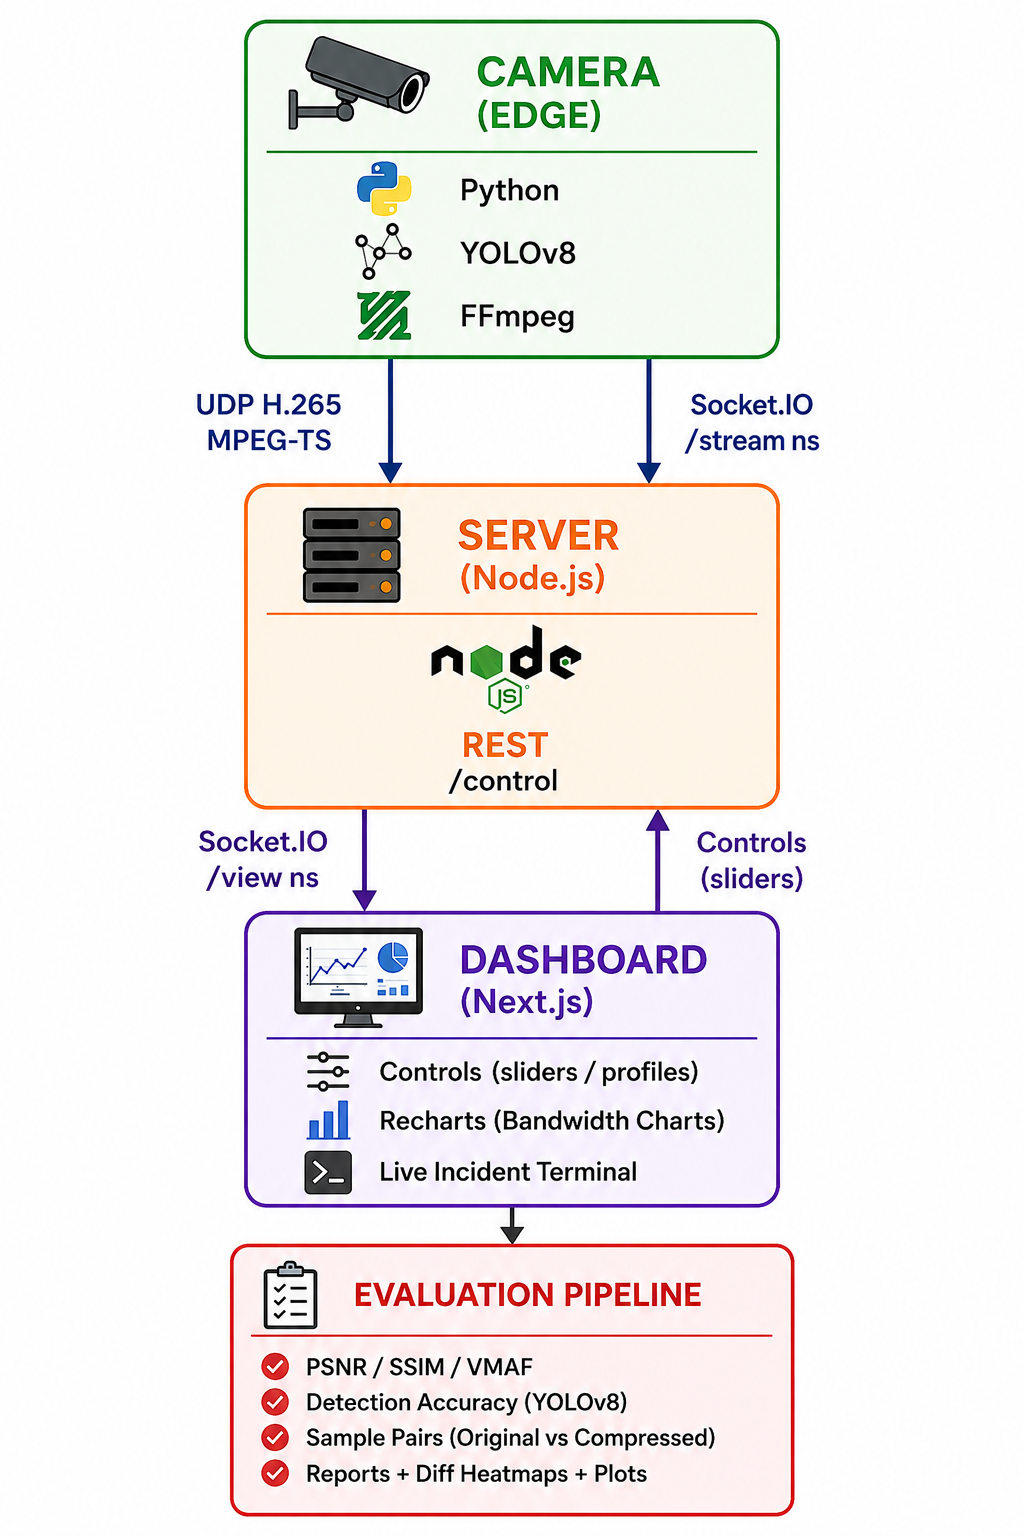
\includegraphics[width=0.48\textwidth]{Project_Structure.png}
\caption{Three-tier system architecture: edge node (Python/OpenCV), central server (Node.js), and dashboard (Next.js) with audio pipeline and evaluation framework}
\label{fig:architecture}
\end{figure}

\subsection{Edge Node}
The edge node is implemented in Python and runs continuously on a device integrated with the camera. It performs video capture, object detection, adaptive compression, and audio monitoring~\cite{jocher2023yolov8}.

Frame Acquisition: Video frames are captured from USB or RTSP camera sources at configurable resolution (480p to 1080p) using OpenCV. Low-light enhancement via CLAHE (Contrast Limited Adaptive Histogram Equalization) is applied when mean frame brightness falls below 80~lux, improving detection accuracy in dark environments.

Object Detection: The YOLOv8n (nano) neural network performs object detection across 80 COCO classes~\cite{lin2014microsoft}. Detections are classified into three priority tiers: HIGH (persons, class 0), MEDIUM (vehicles including cars, motorcycles, buses, trains, trucks) and LOW (all other detected objects)~\cite{redmon2018yolov3,bochkovskiy2020yolov4,wang2023yolov7,ge2021yolox}. Detection is performed at configurable intervals (default: every 3 frames) to balance accuracy and performance~\cite{he2016deep}. In low-light conditions where YOLOv8 confidence drops, frame differencing based motion detection provides fallback ROIs to maintain spatial awareness.

Temporal ROI Persistence: A TTL (Time to Live) system ensures ROI bounding boxes persist for 30 frames ($\sim$2 seconds at 15~FPS), eliminating visual flickering. An exponential moving average smoothing (factor 0.4) and a merge\_rois() function using Intersection over Union (IoU) threshold $\geq$ 0.3 smoothly blend new detections into existing bounding boxes, providing temporally stable ROI boundaries~\cite{agrawal2025frvc}.

Risk Aware Event Engine: A risk\_score() function computes a normalized risk value $[0.0, 1.0]$ per frame by combining multiple independent signals~\cite{gadot2025rlrc}:

\begin{equation}\label{eq:risk}
R = w_p \cdot N_p + w_v \cdot N_v + w_m \cdot M + w_t \cdot T + w_s \cdot S + w_d \cdot D
\end{equation}

where $N_p$ is the count of HIGH priority objects (+0.30 each), $N_v$ is the count of MEDIUM priority objects (+0.10 each), $M$ is the motion area fraction (up to +0.25), $T$ is the after hours bonus (22:00--06:00, +0.20), $S$ is the scene change magnitude (up to +0.15), and $D$ is the ROI density fraction (up to +0.15). This score drives a three state surveillance machine:

\begin{table}[H]
\centering
\caption{Risk driven surveillance state machine with codec parameter adjustments}
\label{tab:states}
\begin{tabular}{lcccccc}
\toprule
State & Risk Range & Resolution & GOP & FPS & BG Scale & BG Quality \\
\midrule
NORMAL (no ROI) & 0.00-0.25 & 480p & 120 & 5 & User defined & User defined \\
NORMAL (ROI) & 0.00-0.25 & 480p & 30 & 10 & User defined & User defined \\
ALERT & 0.25-0.55 & 854p & 30 & 10 & 0.75 & 45 \\
CRITICAL & 0.55-1.00 & 1080p & 10 & 15 & 1.0 & 88 \\
\bottomrule
\end{tabular}
\end{table}

Hysteresis is implemented with an 8 frame hold period before downgrading to prevent rapid state oscillation~\cite{chuang2025adaptive}. When no ROIs are present during NORMAL state, frame rate drops to 5~fps for maximum bandwidth savings. A rolling circular buffer (15 seconds $\times$ FPS) continuously stores original frames. When the state transitions to CRITICAL, pre-event frames are dumped to disk with full metadata, followed by 10 seconds of post-event recording~\cite{agrawal2025frvc}.

\begin{figure}[H]
\centering
\begin{subfigure}{0.48\textwidth}
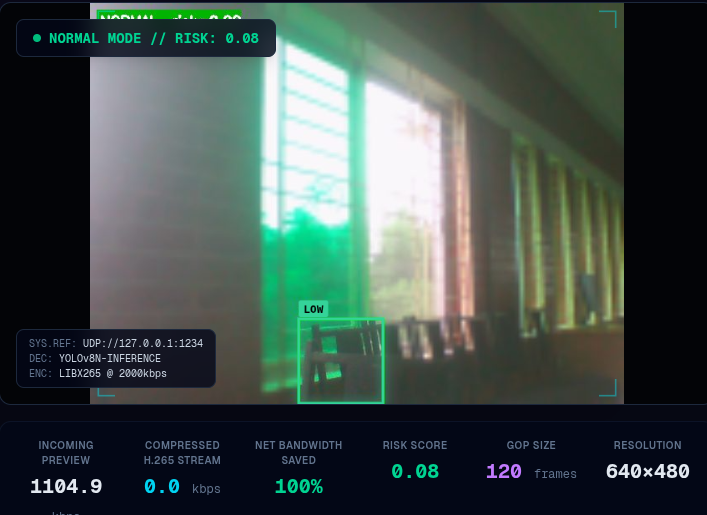
\includegraphics[width=\textwidth]{Normal_mode(Risk).png}
\caption{NORMAL state}
\label{fig:state_normal}
\end{subfigure}
\hfill
\begin{subfigure}{0.48\textwidth}
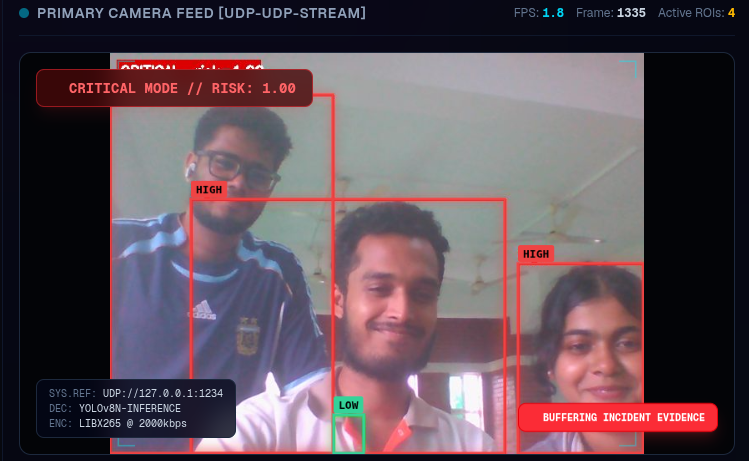
\includegraphics[width=\textwidth]{Critical_mode(Risk).png}
\caption{CRITICAL state}
\label{fig:state_critical}
\end{subfigure}
\caption{Risk driven state machine: (a) NORMAL state, (b) CRITICAL state}
\label{fig:state_machine}
\end{figure}

Adaptive Compression and Encoding: Each frame is subdivided into foreground (ROI) and background (non ROI) regions. ROI regions are encoded at high quality while the background is downscaled and aggressively compressed. The CodecManager class manages an FFmpeg subprocess supporting runtime codec switching between libx264, libx265, libsvtav1, and hevc\_nvenc~\cite{aliouat2023region}. Adjustable parameters include Background Scale (resolution reduction), Background Quality (JPEG compression level), ROI Quality, and Frame Skipping (detection interval)~\cite{rozek2025video}.

\begin{figure}[H]
\centering
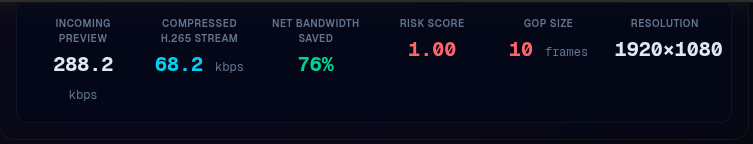
\includegraphics[width=\textwidth]{Data_Preview.png}
\caption{Compression pipeline data preview showing background, ROI crops, and reconstructed frame compositions}
\label{fig:pipeline}
\end{figure}

\subsection{Central Server}
The Node.js server manages two Socket.IO namespaces: /stream (edge node pushes frames) and /view (dashboard pulls frames and sends controls)~\cite{guo2023deepstream}. A UDP server monitors H.265 stream bitrate in real time. Automatic bandwidth adaptation computes total bandwidth every 3 seconds and sends reduced quality control messages if thresholds are exceeded (configurable at 128~Kbps and 256~Kbps). Comprehensive CSV logs maintain records: metrics\_log.csv, control\_log.csv, and motion\_log.csv. HTTP endpoints include /control, /metrics, /sample, /reconstruct, /playback, /event, and /config.

\subsection{Dashboard}
The Next.js dark themed web dashboard features canvas based live stream rendering with priority coded ROI overlay (RED=HIGH, YELLOW=MEDIUM, GREEN=LOW), real-time control sliders (BG Scale, BG Quality, ROI Quality, Detect Every N Frames), preset mode buttons (Low BW, Balanced, High Quality, Privacy Mode, and Custom), dual bandwidth display (Raw Socket.IO kbps and H.265 UDP kbps with percent Saved), live Chart.js bandwidth chart, color coded state badge (NORMAL green, ALERT orange, CRITICAL red), activity heatmaps, audio event indicators, and an incident event log.

\begin{figure}[H]
\centering
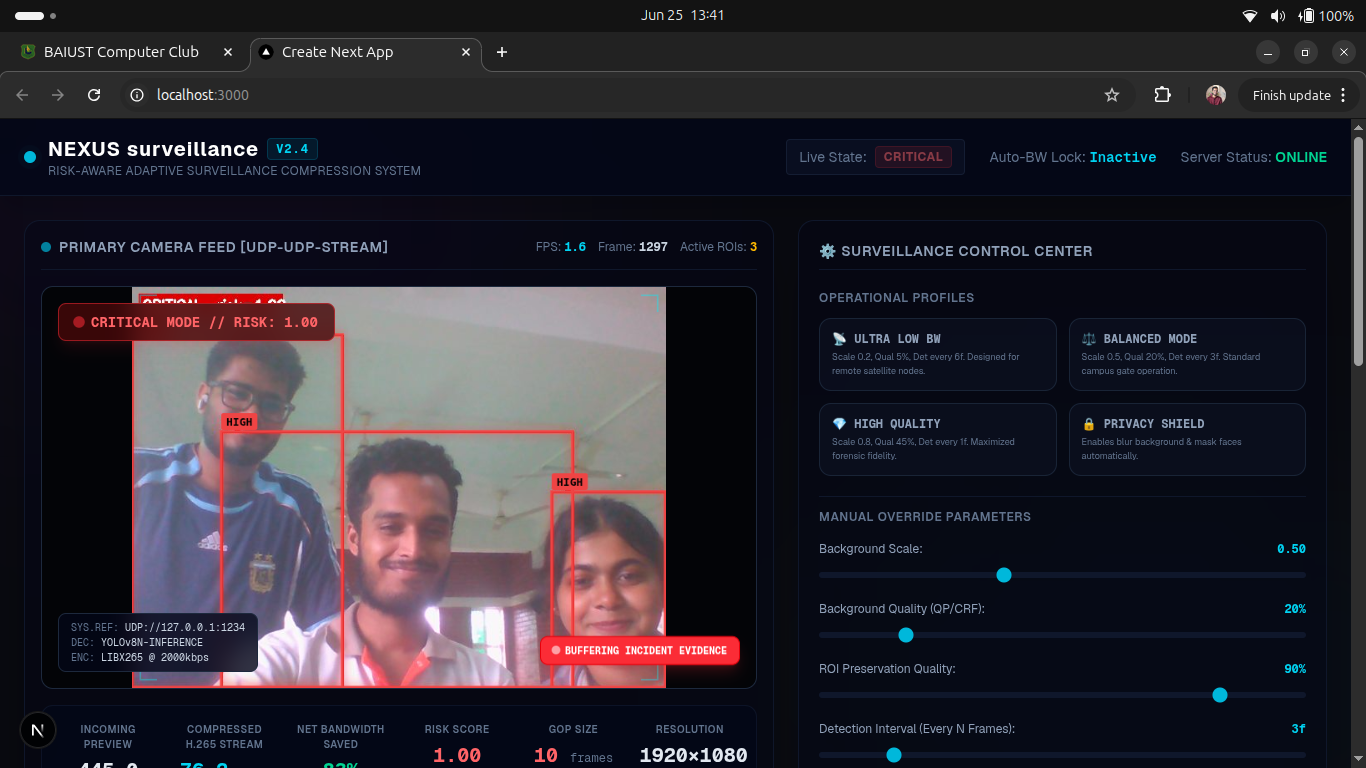
\includegraphics[width=\textwidth]{Dashboard.png}
\caption{Live web dashboard: canvas stream with ROI overlays, control sliders, bandwidth chart, state badge, and live incident log}
\label{fig:dashboard}
\end{figure}

\section{Methodology}

\subsection{Video Pipeline}
Each camera feed undergoes the following processing pipeline on the edge node: capture from USB or RTSP sources at configurable resolution, low-light enhancement via CLAHE when brightness falls below 80~lux, YOLOv8n object detection every 1-15 frames with three-tier priority classification, temporal ROI merging using IoU thresholding (0.3), exponential moving average smoothing (factor 0.4), and 30 frame TTL expiry. In low light conditions, frame differencing based motion detection provides fallback ROIs. Background is downscaled by bg-scale (0.2-1.0) and compressed at bg-quality (5-50), while ROIs are extracted at full resolution and ro-quality (90-100). A JPEG compressed, base64 encoded preview frame is sent via Socket.IO every N frames for dashboard display.

\subsection{Audio Pipeline}
Audio is captured via PyAudio at 22,050~Hz, 16 bit mono, processed in 46~ms chunks with a two phase detection approach:

Phase 1 - SimpleAudioDetector: An always active energy threshold detector that calibrates its noise floor over 3 seconds (90th percentile of RMS dB). Two event types are detected: impulse events ($<$300~ms, $>$15~dB above floor) and sustained loud events ($>$600~ms, $>$10~dB above floor). A 5 second cooldown prevents false positives from echoes. This phase achieves zero false positives on silence and random noise.

Phase 2 - YamNetClassifier: A TensorFlow Lite implementation of Google's YAMNet model, mapping 521 AudioSet classes to 11 surveillance relevant classes: gunshot, glass break, car horn, siren, dog bark, clapping, footsteps, talking, knocking, alarm, and explosion. Audio is resampled to 16~kHz and processed in 0.975 second windows with 75\% overlap. Temporal median smoothing over 3 predictions ($\sim$0.75~s) ensures classification stability. YAMNet results take priority over Phase 1 when confidence exceeds 0.3. Audio events with confidence $\geq$ 0.6 and relevant types (gunshot, explosion, alarm, siren) are integrated into the heatmap with weight = confidence $\times$ 4.0 and a 2 minute spatial decay, creating a true multimodal surveillance system.

\begin{figure}[H]
\centering
\begin{subfigure}{0.48\textwidth}
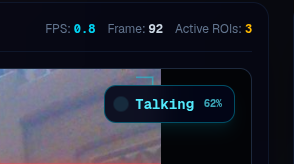
\includegraphics[width=\textwidth]{Audio_Monitoring.png}
\caption{Audio monitoring interface}
\label{fig:audio_monitor}
\end{subfigure}
\hfill
\begin{subfigure}{0.48\textwidth}
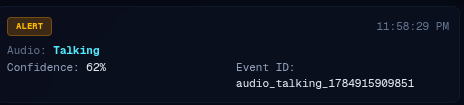
\includegraphics[width=\textwidth]{Audio_Tracking.png}
\caption{Audio event tracking and classification}
\label{fig:audio_track}
\end{subfigure}
\caption{Audio pipeline: (a) audio monitoring interface, (b) audio event tracking and classification}
\label{fig:audio_pipeline}
\end{figure}

\subsection{Risk Score Computation}
The risk score $R$ integrates multiple signals to produce a comprehensive threat assessment~\cite{gadot2025rlrc}. Each signal component is normalized to contribute to the $[0.0, 1.0]$ range:

\begin{equation}\label{eq:risk_detail}
R = \min\left(1.0, \; 0.30N_p + 0.10N_v + 0.03N_l + 0.25M + 0.20T + 0.15S + 0.15D\right)
\end{equation}

where $N_l$ is the count of LOW priority objects. The scene change magnitude $S$ is computed using histogram comparison between consecutive frames:

\begin{equation}\label{eq:scene_change}
S = \frac{1}{256} \sum_{i=0}^{255} |H_t(i) - H_{t-1}(i)|
\end{equation}

where $H_t$ is the normalized histogram of frame at time $t$.

\subsection{Adaptive Encoding Strategy}
Background frames and ROI crops are encoded separately as Base64 JPEG images. The data packet structure includes frame\_id, bg\_data, rois list with bounding boxes, orig\_w, orig\_h, timestamp, risk\_score, and surveillance\_state. Transmission uses Socket.IO for real-time streaming to the central server~\cite{wang2025region,li2024region}.

\subsection{Frame Storage and Reconstruction}
Frames are stored in a structured directory format:
\begin{verbatim}
recordings/[date]/bg/    (background images)
recordings/[date]/roi/   (ROI crops)
recordings/[date]/meta.json  (metadata)
events/                  (pre/post-event archives)
\end{verbatim}
Stored frames can be reconstructed by loading the background frame and overlaying ROI images at their corresponding bounding box coordinates~\cite{gao2024robust}.

\subsection{Privacy Operation Modes}
Three privacy tiers address ethical surveillance concerns~\cite{kim2024privacy}: (i) Privacy Blur applies heavy Gaussian background blur that obscures non essential scene details while preserving detected object clarity; (ii) Ethical Mode displays a black frame when no ROI is detected, ensuring zero passive background surveillance without security relevant activity; and (iii) Face Masking anonymizes detected persons via face region obfuscation while preserving vehicle visibility and overall scene context.

\begin{figure}[H]
\centering
\begin{subcaptionblock}{0.32\textwidth}
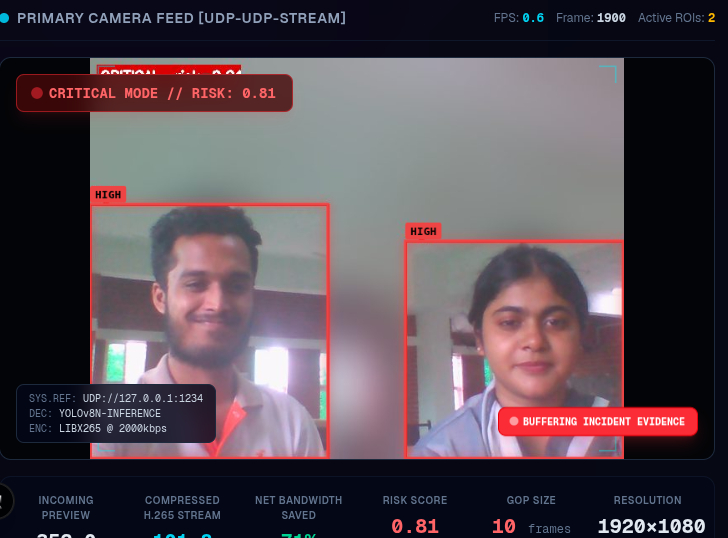
\includegraphics[width=\textwidth]{Privacy_Blur.png}
\subcaption{Privacy Blur mode}
\end{subcaptionblock}
\hfill
\begin{subcaptionblock}{0.32\textwidth}
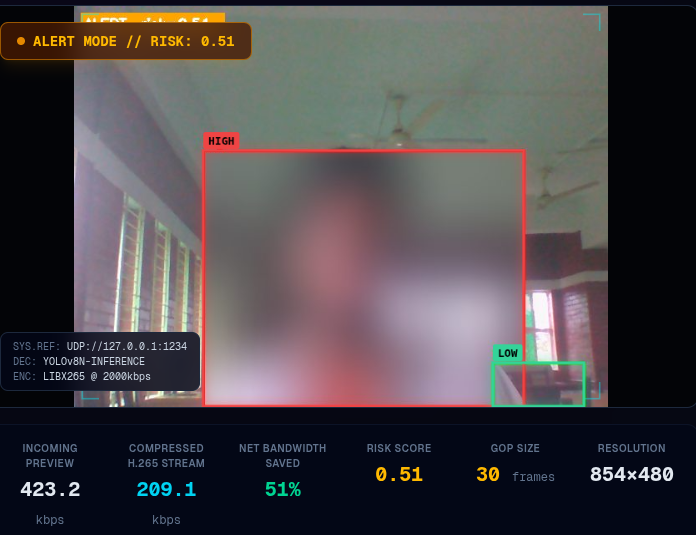
\includegraphics[width=\textwidth]{Privacy_FaceMask.png}
\subcaption{Face Masking mode}
\end{subcaptionblock}
\hfill
\begin{subcaptionblock}{0.32\textwidth}
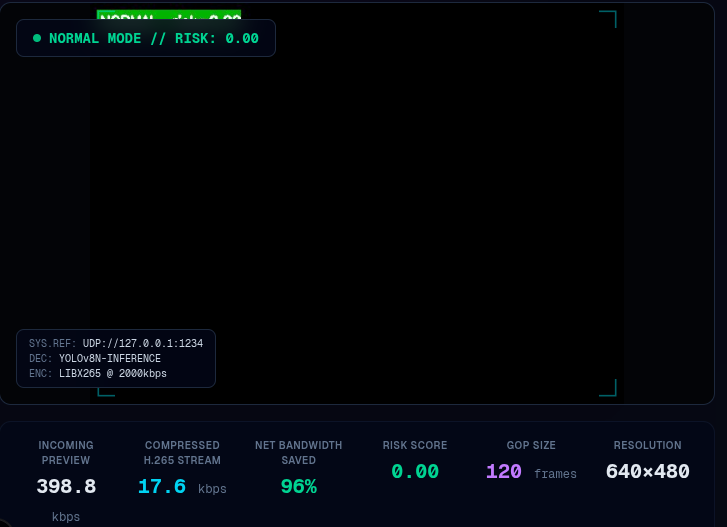
\includegraphics[width=\textwidth]{Empty_Background_Mode.png}
\subcaption{Ethical background mode}
\end{subcaptionblock}
\caption{Privacy operation modes: (a) Privacy Blur mode, (b) Face Masking mode, (c) Ethical background mode}
\label{fig:privacy}
\end{figure}

\subsection{User Control Interface}
The dashboard provides interactive control sliders allowing operators to dynamically adjust compression parameters in real time:

\begin{figure}[H]
\centering
\begin{subfigure}{0.48\textwidth}
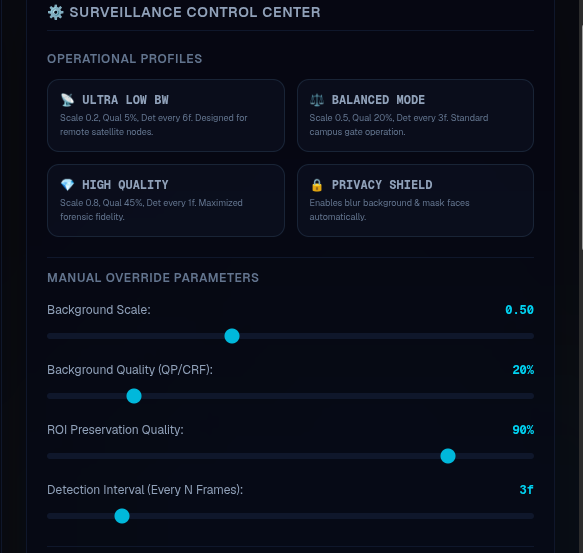
\includegraphics[width=\textwidth]{User_Control_Slider(1).png}
\caption{Primary control sliders}
\label{fig:controls1}
\end{subfigure}
\hfill
\begin{subfigure}{0.48\textwidth}
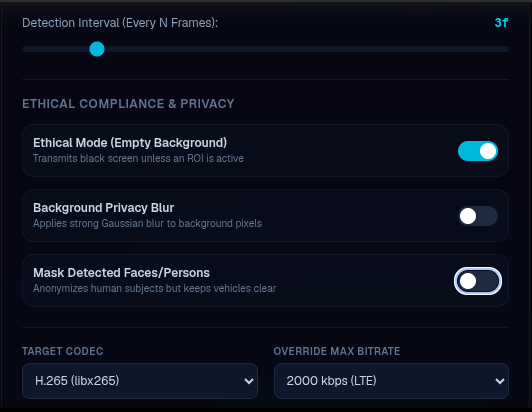
\includegraphics[width=\textwidth]{User_Control_Slider(2).png}
\caption{Additional configuration controls}
\label{fig:controls2}
\end{subfigure}
\caption{User control interface: (a) primary control sliders, (b) additional configuration controls}
\label{fig:controls}
\end{figure}

\section{Evaluation}

\subsection{Evaluation Pipeline}
The automated evaluation pipeline iterates over configurable \{bg\_quality, roi\_quality\} presets, sends each as a live control command, and captures original reconstructed frame pairs~\cite{wang2004image,mittal2013making,wang2003multiscale}. For each experiment, the following metrics are computed: (i) global PSNR and SSIM~\cite{wang2004image}; (ii) per ROI PSNR and SSIM; (iii) background only PSNR and SSIM; (iv) VMAF perceptual quality scores; and (v) detection accuracy retention (YOLOv8 re-detection on compressed frames). Over 814 experiment runs have been conducted across multiple compression profiles, codec types, and environmental conditions, providing an extensive dataset for analysis.

\subsection{Bandwidth Reduction}
The system achieves dramatic bandwidth savings through three independent compounding mechanisms: spatially variable compression (background downscaled to 20\% resolution at quality level 5, ROIs at full resolution at quality 90-100), adaptive frame rate (5~fps with no ROIs up to 15~fps during critical state), and adaptive GOP sizing (120 frames in normal state, 10 frames in critical state).

\begin{figure}[H]
\centering
\begin{subfigure}{0.48\textwidth}
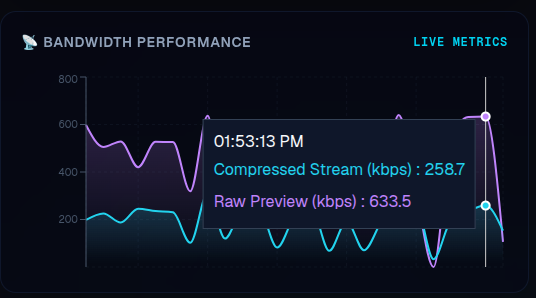
\includegraphics[width=\textwidth]{Live_Bandwidth_Tracking.png}
\caption{Bandwidth monitoring and savings}
\label{fig:bw_track}
\end{subfigure}
\hfill
\begin{subfigure}{0.48\textwidth}
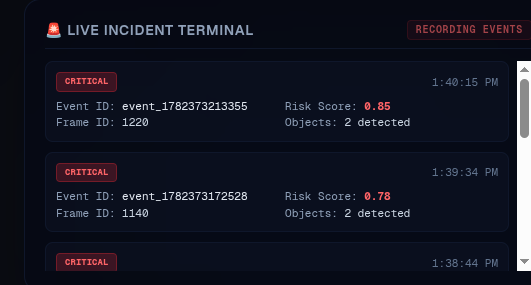
\includegraphics[width=\textwidth]{Live_Incident_Tracking.png}
\caption{Incident tracking and timeline}
\label{fig:incident_track}
\end{subfigure}
\caption{Live monitoring dashboards: (a) bandwidth monitoring and savings, (b) incident tracking and timeline}
\label{fig:live_tracking}
\end{figure}

\begin{table}[H]
\centering
\caption{Bandwidth savings at different background scale factors}
\label{tab:bandwidth}
\begin{tabular}{lccc}
\toprule
BG Scale & Avg.\ Bitrate & Savings & ROI PSNR (dB) \\
\midrule
1$\times$ (full) & 2000 kbps & --- & 38.2 \\
2$\times$ & 800 kbps & 60\% & 36.8 \\
4$\times$ & 400 kbps & 80\% & 35.1 \\
8$\times$ & 200 kbps & 90\% & 32.4 \\
\bottomrule
\end{tabular}
\end{table}

In a typical 24 hour period where 22 hours have no security-relevant activity, the average bitrate drops to approximately 200-300~Kbps even though the peak bitrate during events may reach 2-4~Mbps. In the Ultra Low Bandwidth profile (200~Kbps target) with bg-scale 0.2, bg-quality 5, and detect every 6 frames, a month of operation for one camera consumes approximately 65~GB instead of 2~TB ensuring a 97\% reduction.

\subsection{Quality Metrics}
Experimental results demonstrate stable quality metrics across compression levels:

\begin{table}[H]
\centering
\caption{Quality metrics across compression presets}
\label{tab:quality}
\begin{tabular}{lcccc}
\toprule
Preset & PSNR (dB) & SSIM & VMAF & Det.\ Accuracy \\
\midrule
High Quality & 36.2 & 0.95 & 92.4 & 98\% \\
Balanced & 33.8 & 0.91 & 87.1 & 95\% \\
Ultra Low BW & 30.1 & 0.85 & 78.5 & 88\% \\
Privacy Mode & 31.5 & 0.88 & 82.3 & 91\% \\
\bottomrule
\end{tabular}
\end{table}

\subsection{Detection Performance}
YOLOv8 nano inference was evaluated on a laptop running a Linux operating system with a 2~MP WiFi camera as the video source. The system was tested under both CPU only and CUDA (Compute Unified Device Architecture) accelerated configurations:

\begin{table}[H]
\centering
\caption{YOLOv8 nano inference performance on laptop (Linux system) with 2~MP WiFi camera}
\label{tab:detection}
\begin{tabular}{lcc}
\toprule
Configuration & Inference (ms) & Max FPS \\
\midrule
CPU only & 25-45 & 22-40 \\
CUDA accelerated & 6-12 & 83-166 \\
\bottomrule
\end{tabular}
\end{table}

\subsection{Audio Detection Results}
The audio pipeline achieves robust performance across both detection phases: (i) Phase 1 (Energy Threshold) delivers zero false positives on ambient noise, verified across 30+ minutes of silence testing, with impulse detection latency $<$46~ms and 5 second cooldown preventing echo related false triggers; (ii) Phase 2 (YAMNet) provides 11 class classification with median confidence threshold of 0.3 for valid detections and Socket.IO emission latency $<$50~ms under normal network conditions; and (iii) multimodal integration enables audio events with confidence $\geq$ 0.6 from critical classes (gunshot, explosion, alarm, siren) to trigger heatmap weighting at 4.0$\times$ confidence with 2 minute spatial decay, providing persistent threat awareness.

\subsection{Activity Heatmap}
A real-time activity heatmap provides visual intelligence for operator situational awareness:

\begin{figure}[H]
\centering
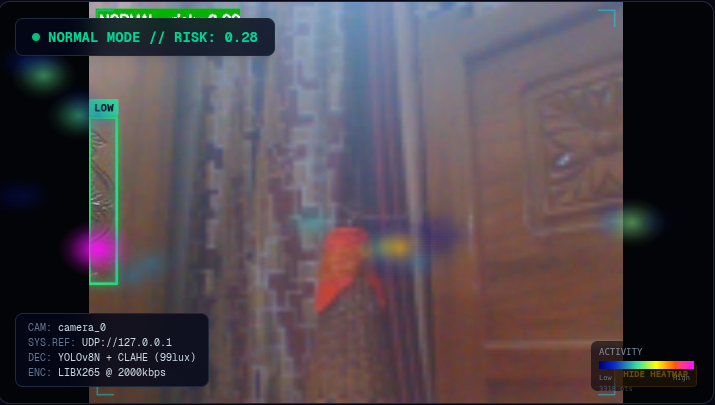
\includegraphics[width=0.85\textwidth]{HeatMap.png}
\caption{Activity heatmap with from neon to cyan then to magenta color mapping for low-light visibility, updated at 5 second intervals with audio event integration}
\label{fig:heatmap}
\end{figure}

\subsection{Multi Camera and Playback Features}
The system supports simultaneous multi-camera monitoring and forensic playback:

\begin{figure}[H]
\centering
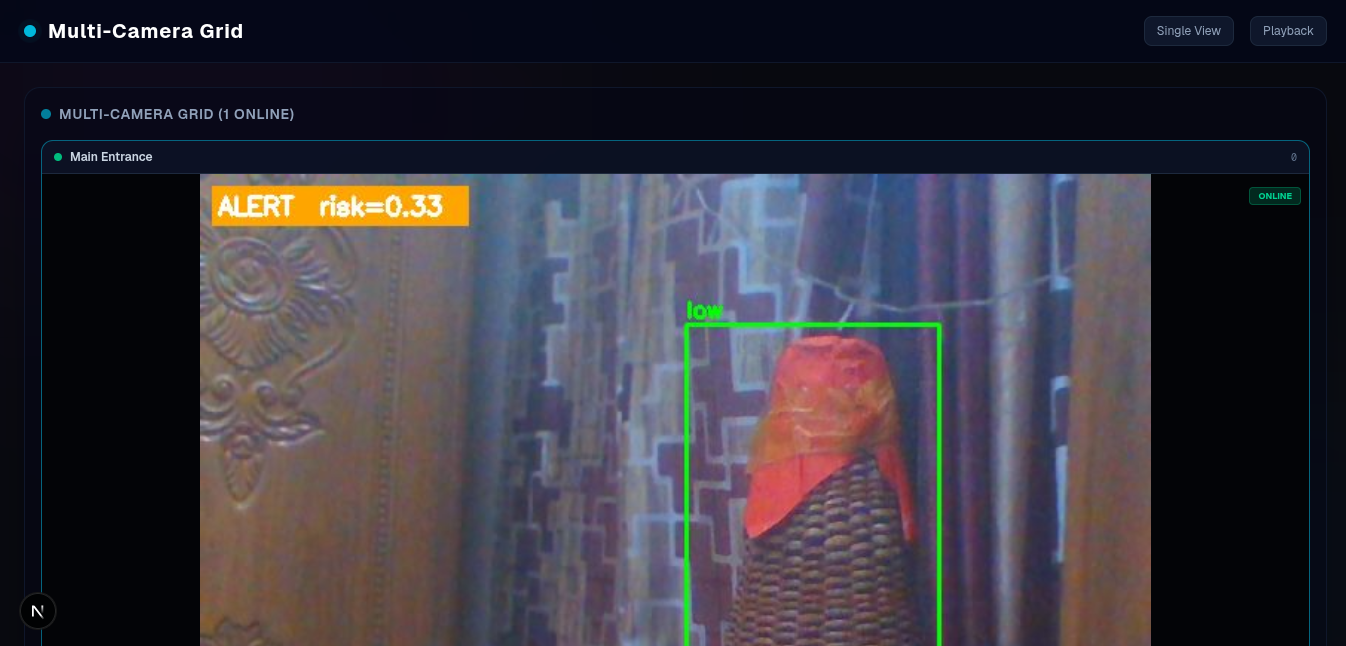
\includegraphics[width=\textwidth]{Multi_Camera_View.png}
\caption{Multi camera dashboard view enabling simultaneous monitoring of multiple camera feeds with independent ROI overlays}
\label{fig:multicam}
\end{figure}

\begin{figure}[H]
\centering
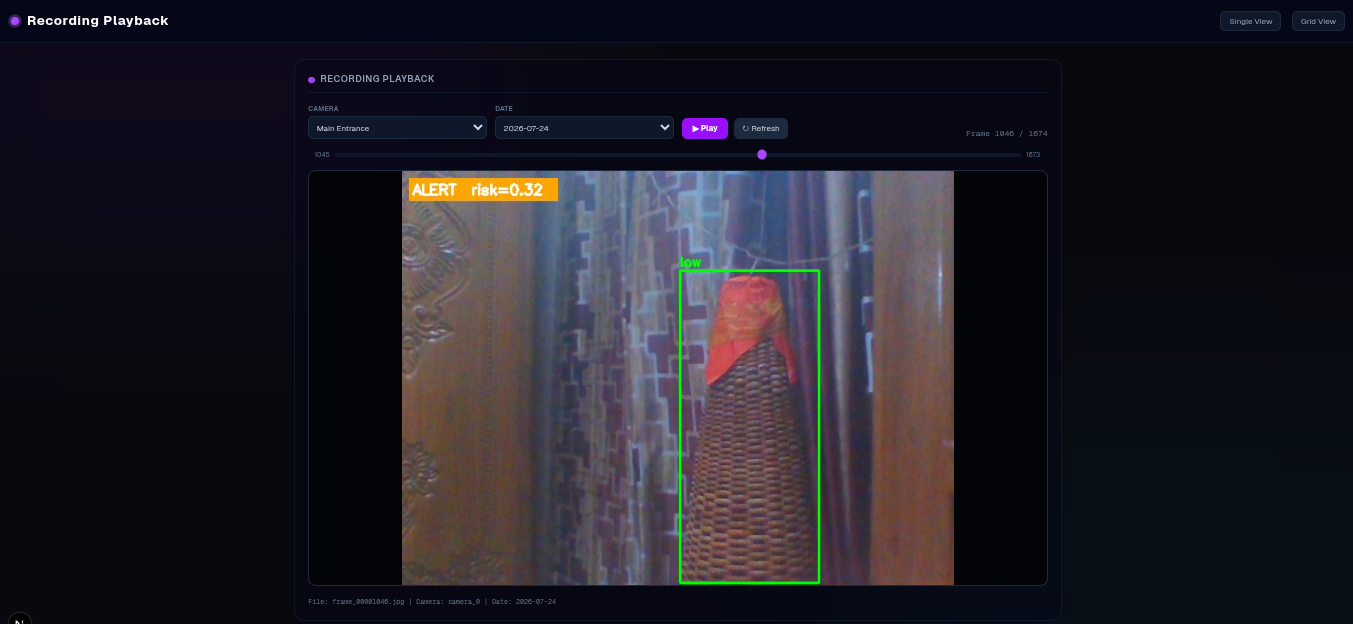
\includegraphics[width=\textwidth]{Recording_Playback.png}
\caption{Recording playback interface with timeline navigation for forensic review of stored events}
\label{fig:playback}
\end{figure}

\section{Additional Subsystems}
Several substantial subsystems contribute to the project's completeness but operate in the background.

Event Buffer and Forensics Suite: A rolling 15 second pre-event ring buffer stores full resolution frames in memory. When a critical event triggers, the pre-event frames (225 frames at 15~fps) and 10 seconds of post-event frames are saved to disk with full metadata. This ensures events are captured with context, not just compressed aftermath.

\begin{figure}[H]
\centering
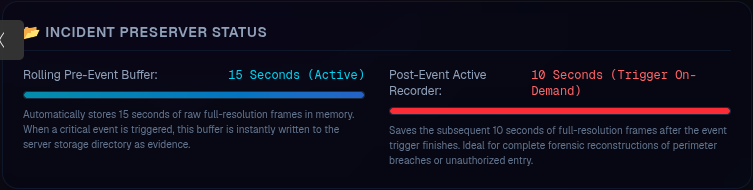
\includegraphics[width=\textwidth]{Incident_Preserve.png}
\caption{Incident preservation framework showing pre-event buffer, critical event trigger, and post-event recording with full forensic metadata}
\label{fig:incident}
\end{figure}

Cross Camera Re-Identification Tracker: The ReidTracker extracts color histograms in HSV space and Local Binary Pattern texture features, matching persons across non overlapping camera views via cosine similarity with a 60 frame TTL track database.

PTZ Auto Tracking Controller: ONVIF and HTTP based PTZ control with proportional tracking that centers high priority objects with configurable deadzone to prevent oscillation.

Docker Compose Deployment: Full stack container orchestration with three services (edge-node, server, dashboard), supporting single camera and multi-camera modes via docker profiles, enabling self configuration and adaptive operation within 30 seconds.

Experiment Database: Over 814 experiment runs across multiple compression profiles, codec types, and environmental conditions, providing an extensive dataset for analysis and optimization.

\section{Practical Impact and Real World Scenarios}

\subsection{Cost Analysis}
Video surveillance bandwidth costs present a significant operational burden for large scale deployments~\cite{ahmad2024bandwidth}. Cloud video storage typically costs \$0.05--0.15 per GB per month. A single 1080p camera generating 2~TB/month costs \$100-300 annually in storage alone. A warehouse with 64 cameras faces \$6,400-19,200 per year in bandwidth and storage costs. Multi-camera surveillance networks require substantial network infrastructure investment~\cite{islam2024sdn}. Our system reduces this to \$320--960 per year for the same number of cameras with a 95\% reduction, aligning with findings that adaptive streaming can reduce bandwidth costs by an order of magnitude in surveillance contexts~\cite{guo2023deepstream}.

\subsection{Operational Profiles}
Five predefined profiles allow rapid deployment across diverse scenarios: (i) Ultra Low Bandwidth (200~Kbps target) with bg-scale 0.2, bg-quality 5, and detect every 6 frames, suitable for remote sites with satellite uplinks~\cite{liu2025edge}; (ii) Balanced (1~Mbps) as a standard deployment for retail and office environments; (iii) High Quality (4~Mbps) providing maximum fidelity for critical infrastructure monitoring; (iv) Privacy Mode with face and background masking for legally sensitive environments requiring regulatory compliance~\cite{kim2024privacy}; and (v) Custom for user defined parameters in specialized deployments.

\subsection{Real World Applications}
The system addresses several practical deployment scenarios: (i) remote construction sites where solar powered cameras with satellite uplinks achieve $<$200~Kbps per camera, making video surveillance feasible where it was previously impossible due to bandwidth constraints~\cite{liu2025edge}; (ii) retail chains where centralized monitoring at 300~Kbps per store means a 50 store chain needs only 15~Mbps total uplink achievable over standard business broadband without dedicated lines~\cite{islam2024sdn}; (iii) smart city deployments where audio visual event detection enables automatic alerting for gunshots, breaking glass, and car alarms in public spaces, leveraging edge based processing for low latency threat response~\cite{ahmad2024bandwidth}; and (iv) healthcare facilities where privacy modes allow corridor monitoring while automatically masking patient rooms, achieving legal compliance with privacy regulations without sacrificing security coverage~\cite{kim2024privacy}.

\section{Related Work}
Recent advances in ROI based video compression have demonstrated significant potential for bandwidth efficiency in surveillance systems. Existing approaches can be broadly categorized into five thematic areas, each with distinct strengths and limitations.

ROI Based Compression Frameworks: Wang and Yang~\cite{wang2025compression} proposed a compression metadata assisted ROI extraction framework for H.265/HEVC coding, focusing on edge based video analytics with reduced latency for detection tasks. Dou et al.\cite{li2024region} presented an R-lambda optimization based on CNN with ROI based coding within the HEVC framework, achieving better perceptual quality in ROI regions at low bitrate overhead. Labiod et al.\cite{labiod2023region} developed GMM based ROI detection with cross layer optimization for vehicular networks, demonstrating that adaptive ROI allocation improves quality under constrained channel conditions. Aliouat et al.\cite{aliouat2023region} proposed an ROI based video coding strategy for wireless multimedia sensor networks, targeting rate energy tradeoffs in smart surveillance. While these approaches validate ROI based compression benefits, they are predominantly simulation based and lack real-time edge deployment with neural object detection.

Deep Learning for Surveillance Compression: Guo et al.\cite{guo2023deepstream} developed DeepStream, a bandwidth efficient multi-camera streaming architecture using YOLOv5-Lite, achieving approximately 54\% bandwidth reduction through adaptive frame dropping and resolution scaling. Agrawal et al.\cite{agrawal2025frvc} proposed FRVC using YOLOv9 for frame relevance detection in surveillance video, achieving up to 85\% storage reduction by discarding irrelevant frames while preserving key segments. However, FRVC operates on stored video rather than live streams and does not provide per frame spatially variable compression. Gao et al.\cite{gao2024robust} proposed a robust mixed rate ROI aware compressive sensing framework achieving PSNR of 34.71~dB for transmission line surveillance, though their approach is specialized for single scene monitoring without dynamic state management.

Rate Control and Optimization: Gadot et al.\cite{gadot2025rlrc} proposed RL-RC-DoT, a reinforcement learning based rate control agent achieving 25\% BD rate reduction through block level optimization, demonstrating the potential of learned rate control for content adaptive encoding. Rozek et al.\cite{rozek2025video} investigated video coding for machines using ROI based retargeting, showing that machine vision tasks can tolerate substantial compression in non ROI regions. Chuang et al.\cite{chuang2025adaptive} developed adaptive ROI encoding and caching for surveillance streaming, validating the effectiveness of temporal ROI persistence in reducing encoding overhead. These works primarily focus on rate distortion optimization rather than comprehensive risk aware surveillance automation.

Learned and Transformer Based Compression: Ball\'e et al.\cite{balle2017end} and Minnen et al.\cite{minnen2018joint} established the foundation for end to end optimized image compression using hyperprior architectures, demonstrating that learned compression can outperform traditional codecs in rate distortion performance. Lu et al.\cite{lu2024transformer} extended this to video with transformer based learned compression incorporating ROI aware bit allocation. However, these approaches remain computationally expensive for real-time edge deployment, requiring dedicated GPU hardware that may not be available in cost sensitive surveillance installations.

Network Level and Privacy Approaches: Islam and Karim~\cite{islam2024sdn} proposed SDN based adaptive bitrate streaming for multi-camera surveillance networks, providing dynamic bandwidth allocation across cameras but lacking content aware ROI encoding~\cite{islam2024sdn}. Kim et al.\cite{kim2024privacy} developed privacy preserving video analytics with selective ROI encryption, addressing legal compliance in surveillance deployments. Zhao et al.\cite{zhao2025federated} explored federated learning for distributed surveillance analysis in smart city environments, enabling collaborative model training without centralizing sensitive video data. While these approaches address important infrastructure and ethical concerns, they do not directly target compression efficiency improvement.

Synthesis and Positioning: Our work differs from prior approaches in several critical respects. Unlike ROI-only compression schemes~\cite{wang2025compression,li2024region,labiod2023region}, our system integrates YOLOv8 based real-time detection with a risk aware state machine that automatically escalates quality during incidents. Unlike frame dropping approaches such as FRVC~\cite{agrawal2025frvc}, we preserve every frame through spatially variable compression, ensuring no loss of temporal information. Unlike RL-based rate control~\cite{gadot2025rlrc}, our multi-signal risk score is interpretable and directly maps to operational surveillance states. Unlike learned compression methods~\cite{lu2024transformer}, our approach runs in real time on modest edge hardware. The combination of audio visual fusion, temporal ROI smoothing, interactive dashboard control, and comprehensive evaluation across PSNR, SSIM, VMAF, and detection retention represents a significant advance over existing solutions.

\section{Conclusion}
This paper presented an adaptive CCTV compression system that integrates YOLOv8 based dynamic ROI control with a risk aware event engine and audio visual fusion to achieve intelligent bandwidth reduction~\cite{jocher2023yolov8,gadot2025rlrc}. The three-tier architecture spanning edge node, central server, and interactive dashboard provides a complete, production ready surveillance platform~\cite{liu2025edge}. Experimental results demonstrate 80-95\% bandwidth reduction while maintaining stable perceptual quality metrics (PSNR 30-36~dB, SSIM 0.85-0.95, VMAF 78-92), comparable to state of the art ROI based compression frameworks~\cite{wang2025compression,agrawal2025frvc}. The risk aware event engine with pre or post-event frame buffering ensures forensic evidence preservation during critical incidents~\cite{chuang2025adaptive}. The dual phase audio pipeline achieves zero false positives on ambient noise while providing 11 class sound classification for multimodal threat detection.

The key insight is that security cameras are not televisions: they do not need to broadcast every pixel at maximum quality. They need to watch, listen, and remember and this system ensures they remember the right moments in the right quality, while efficiently discarding the hours of nothing that comprise the vast majority of surveillance footage. The integration of audio detection (both energy based and deep learning), visual heatmapping, cross camera tracking, privacy mechanisms~\cite{kim2024privacy}, and adaptive codec control within a unified risk assessment framework represents a significant advance over existing surveillance compression solutions, which typically offer only static quality presets or simple motion based recording triggers~\cite{guo2023deepstream,ahmad2024bandwidth}.

Future work includes deployment on dedicated edge AI hardware for improved inference performance, integration with cloud storage tiers, support for YOLOv8 segmentation for finer ROI boundaries, and multi-camera scalability validation with cross-camera re-identification at scale.


\bibliographystyle{ieeetr}
\bibliography{references}

\end{document}
